%\documentclass{kuisthesis}			% 特別研究報告書
%\documentstyle[master]{kuisthesis}		% 修士論文(和文)
%\documentclass[master]{kuisthesis}		% 修士論文(和文)
%\documentstyle[master,english]{kuisthesis}	% 修士論文(英文)
\documentclass[master,english]{kuisthesis}	% 修士論文(英文)

\usepackage[a4paper]{geometry}

% \usepackage{multibib}
\usepackage[dvipdfmx]{graphicx}
\usepackage[dvipdfmx,dvipsnames]{xcolor}
\usepackage{tabularx}
\usepackage{caption}     % \captionsetup

\makeatletter
\let\subfigure\relax
\let\endsubfigure\relax
\let\subtable\relax
\let\endsubtable\relax
\makeatother

\usepackage{titlesec}
\titleformat{\section}[hang]
  {\normalfont\Large\bfseries}
  {Chapter~\thesection}
  {1em}
  {}

\let\KUsec\section
\renewcommand{\section}{\clearpage\KUsec}

\usepackage{subcaption}
% \usepackage{soul}
% \usepackage[latin1]{inputenc}
% \usepackage{xstring}
\usepackage{natbib}
% \usepackage{breakcites}
% \usepackage{siunitx}
% \usepackage{makecell}
% \usepackage{diagbox} % for diagbox
% \usepackage{multirow}
% \usepackage{pdfpages}
\usepackage[ruled,linesnumbered,vlined]{algorithm2e}
% \usepackage{amsmath}
\usepackage{amssymb}
\usepackage{amsthm}
\usepackage{mathtools}
\usepackage{bbm}
\usepackage{booktabs} % To thicken table lines
% \usepackage{verbatim}
\usepackage{multicol}
\usepackage{float}
\usepackage[english]{babel}
\usepackage{amsfonts}
% \usepackage{arydshln}
% \usepackage{subcaption}
% \usepackage{colortbl}
\usepackage[dvipdfmx]{hyperref}
% \usepackage{longtable}

\usepackage{newtxtext}
% \usepackage{newtxmath}
\usepackage{physics}

\input{math_commands.tex}
\newcolumntype{s}{>{\hsize=.5\hsize}X}
% \newcommand{\heading}[1]{\multicolumn{1}{c}{#1}}

% \newcommand{\fn}[1]{\footnote{#1}}
% \renewcommand{\floatpagefraction}{.95}
% %\newcommand{\citept}[1]{\newcitep{#1}}
% %\newcommand{\citep}[1]{\citep{#1}}
% \newcommand{\FIXME}[1]{\fbox{$\star$} (#1)}
% \newcommand{\Sec}[1]{Section~\ref{sec:#1}}
% \newcommand{\Fig}[1]{Figure~\ref{fig:#1}}
% \newcommand{\Tab}[1]{Table~\ref{tab:#1}}
% \newcommand{\Algo}[1]{Algorithm~\ref{algo:#1}}
% \newcommand{\Eq}[1]{Eq.~(\ref{eq:#1})}
% \newcommand{\ra}{{$\rightarrow$}}
% \newcommand{\task}[2]{\mbox{#1{\ra}#2}}


\definecolor{cR}{RGB}{255,204,204}
\definecolor{cG}{RGB}{204,255,204}
\definecolor{cB}{RGB}{204,204,255}
\definecolor{cK}{RGB}{221,221,221}
\definecolor{navyblue}{rgb}{0.0,0.0,0.5}
\newcommand{\bgR}[1]{\cellcolor{cR}#1}
\newcommand{\bgG}[1]{\cellcolor{cG}#1}
\newcommand{\bgB}[1]{\cellcolor{cB}#1}
\newcommand{\bgK}[1]{\cellcolor{cK}#1}
\newcommand{\bgZ}[1]{#1}
\newcommand{\newblock}{}

\newcommand{\uproman}[1]{\uppercase\expandafter{\romannumeral #1}}
\newcommand{\ul}{\underline{\lambda}}
\newcommand{\uL}{\underline{L}}
% \newcommand{\argmax}{\mathop{\rm arg~max}\limits}
% \newcommand{\argmin}{\mathop{\rm arg~min}\limits}
% \newcommand{\mX}{\mathcal{X}}
% \newcommand{\mY}{\mathcal{Y}}

\newcommand{\honda}[1]{\textcolor{red}{[Honda: #1]}}
\newcommand{\nn}{\nonumber\\}
\newcommand{\n}{\nonumber}
\newcommand{\nec}{\mathcal{A}}
\usepackage{comment}
%\newcommand{\id}{ \mbox{\rm 1}\hspace{-0.63em}\mbox{\rm \small 1\,}}
%\newcommand{\idx}[1]{\id\!\left[#1\right]}
\newcommand{\rmax}{i'}

\definecolor{G}{RGB}{142,207,201}
\definecolor{SG}{RGB}{0,251,0}
\definecolor{O}{RGB}{255,190,122}
\definecolor{Y}{RGB}{255,190,122}
\definecolor{R}{RGB}{250,127,111}
\definecolor{SR}{RGB}{250,0,0}
\definecolor{B}{RGB}{130,176,210}
\definecolor{P}{RGB}{190,184,220}

%\usepackage[hidelinks]{hyperref} %% turned off to avoid errors for multi-page hyperlink
\hypersetup
{
    colorlinks=true,
    citecolor=navyblue,
    linkcolor=navyblue,
    filecolor=navyblue,
    urlcolor=navyblue,
}
\urlstyle{same}

\theoremstyle{plain}
\newtheorem{theorem}{Theorem}
%\newtheorem{theorem}{Theorem}[section]
\newtheorem{proposition}[theorem]{Proposition}
\newtheorem{lemma}[theorem]{Lemma}
\newtheorem{corollary}[theorem]{Corollary}
\newtheorem{remark}{Remark}
\theoremstyle{definition}
\newtheorem{definition}[theorem]{Definition}
\newtheorem{assumption}[theorem]{Assumption}
\theoremstyle{remark}

\def\dqed{\tag*{$\square\kern2mm$}} %qed symbol for equations
\newenvironment{proofof}[1]{\par\noindent{\bf #1\ }}{\hfill\BlackBox\\[2mm]} %environment for "Proof of..."
\newenvironment{proof2}{\par\noindent{\bf Proof\ }}{\vspace{0mm}} %without qed symbol
\newenvironment{proofof2}[1]{\par\noindent{\bf #1\ }}{\vspace{0mm}} %combination of the above

\jtitle[知識グラフ埋め込みにおける予測多重性の関係レベル分析]
{知識グラフ埋め込みにおける予測多重性の関係レベル分析}
\etitle[Relation-Level Predictive Multiplicity in Knowledge Graph Embeddings]{Relation-Level Analysis of Predictive Multiplicity in Knowledge Graph Embedding Based Link Prediction}
\jauthor{趙 怡名}         % 和文著者名
\eauthor{Yiming Zhao} % 英文著者名
\supervisor{Prof. Hidetoshi Shimodaira}	% 指導教官名
\date{\today}		% 提出年月日
\department{Systems Science}		% 修士論文の場合の専攻名

\begin{document}
\maketitle                  % とびらの出力

% \begin{jabstract}
%     abstract in Japanese
% \end{jabstract}

\begin{eabstract}
A knowledge graph stores facts as triples that link two objects through a
relation, such as \texttt{(Paris, capital\_of, France)}.
Knowledge graph embedding (KGE) models represent these objects and relations as
vectors and rank candidate objects to complete triples with a missing entry.
Previous work has shown that repeated runs of the same KGE method, trained with
the same configuration but different random seeds, can achieve similar overall
accuracy. Despite this similarity, that work found that, for the same
incomplete triple, one trained model may rank the correct answer among the top
ten candidates while another does not. This disagreement between similarly
accurate models is called predictive multiplicity. It means that an individual
prediction can depend on the random seed used during training even when
aggregate accuracy is stable. However, the analysis in that work summarized
instability mainly over entire test sets, leaving unclear whether some kinds of
relations are more affected than others. Such an overall measurement cannot
show which predictions are more likely to change when the model is retrained,
making it difficult to focus future efforts to improve stability on the most
affected queries.

To address this limitation, this thesis classifies the relations in the dataset
in three ways and compares predictions for the resulting groups in terms of
top-10 accuracy and predictive multiplicity. We refer to these three
classifications as relation patterns. The experiments use FB15k-237, a
benchmark knowledge graph dataset, and two KGE methods, RotatE and TransE. Each
method is evaluated separately through repeated runs with the same
configuration but different random seeds. The first classification, called
mapping type, groups relations as one-to-one, one-to-many, many-to-one, or
many-to-many. For example, \texttt{born\_in} is many-to-one because many people
may share the same birthplace, while each person normally has one birthplace.
The second classification asks whether another relation expresses the same
fact in reverse (inverse), as \texttt{parent\_of} and \texttt{child\_of} do.
The third asks whether the same relation holds in both directions (symmetry),
as \texttt{sibling\_of} does. The clearest difference appears for mapping type.
In both methods, predictions have lower top-10 accuracy and vary more across
repeated runs when many different objects can be linked to the known
object---for example, when predicting a person from a known birthplace. Only a
small group of relations with clear inverse partners is more stable, while
symmetry shows no clear difference in stability. These results show that
classifying relations can reveal differences in prediction stability that are
hidden by overall accuracy.
\end{eabstract}

\tableofcontents			% 目次の出力

\section{Introduction}
\label{chap:introduction}

% TODO（第1段：研究背景）：从 knowledge graphs 和 KGE-based link
% prediction 的大方向开始，说明 link prediction 的基本任务和实际意义。
% 这里只建立研究背景，不提前展开模型公式、数据集或实验流程。

% TODO（第2段：问题引入）：说明 KGE link prediction 通常使用 Hits@10 等
% aggregate metrics 评价总体准确率，但这些指标不能说明总体表现相近的模型
% 是否会对同一个 query 给出相同的 top-10 decision。

% TODO（第3段：已有研究与研究缺口）：引入 predictive multiplicity，说明
% 已有研究已经观察到 query-level prediction instability，但主要在 global
% model level 汇总。由此提出本文的问题：这种不稳定性是否会随不同的
% relations 和 relation patterns 而变化。

% TODO（第4段：本文工作与贡献）：简要说明本文在 FB15k-237 上分析 RotatE
% 和 TransE 的 repeated runs，并比较 relation-level Hits@10、ambiguity 和
% discrepancy。贡献的证据强度要与第5章一致：mapping type 是主要结果；
% inverse 是探索性副结果；symmetry 是弱结果或负结果。不要把本文写成提出
% 新 KGE model 或 multiplicity mitigation method，也不要在这里堆叠具体数字。

% TODO（第5段：论文结构）：在第2至第4章的最终结构稳定后，简要说明各章
% 的功能。避免逐个小节罗列，只说明 background、related work、analysis
% design、experiments 和 conclusion 之间的关系。

\section{Background}
\label{chap:background}

\subsection{Knowledge Graphs and Link Prediction}

% TODO：介绍 entity、relation、triple 和 knowledge graph 的基本定义，并用
% missing-head query 与 missing-tail query 说明 link prediction。解释模型如何
% 对 candidate entities 排序，但暂时不引入 predictive multiplicity。

\subsection{Knowledge Graph Embedding Models}

% TODO：说明 KGE 如何表示 entities 和 relations，以及 scoring function 如何
% 用于 candidate ranking。只介绍后文理解 TransE、RotatE 和实验评估所需要的
% 训练与预测逻辑，不在这里放 hyperparameters。

\subsubsection{TransE}

% TODO：用简单公式介绍 translation-based scoring idea 和本文使用的 score。
% 如果讨论表达能力或局限，必须有对应文献，并且只保留与后文有关的内容。

\subsubsection{RotatE}

% TODO：介绍 complex space 中的 relation rotation 和本文使用的 score。与
% relation patterns 的联系只写原论文明确支持的 representational capacity，
% 不提前暗示这些 patterns 会降低 multiplicity。

\subsection{Link Prediction Evaluation}

% TODO：说明 candidate ranking、raw 与 filtered evaluation 的区别，以及
% Hits@10 的计算和解释。明确 Hits@10 是 aggregate accuracy metric；关于
% query-level instability 的完整讨论留到第3章。

\subsection{Relation Patterns in Knowledge Graph Embeddings}

% TODO：先说明 relation patterns 是 KGE 文献中分析模型表达能力和知识图谱
% 结构的既有视角，不是本文临时创造的分类。区分两类常见描述：基于 relation
% cardinality 的 mapping type，以及 symmetry、antisymmetry、inversion 和
% composition 等 algebraic or logical patterns。表述重点应是 scoring functions
% 能否表示这些 patterns，不要写成模型本身“满足”知识图谱中的数学性质。
% 本文统一使用 relation patterns 作为总称，也不要在这里预设某一种 pattern
% 一定会降低 predictive multiplicity。

\subsubsection{Mapping Type}

% TODO：介绍 1-1、1-N、M-1 和 M-N，以及 average heads per tail、average
% tails per head 和 Bordes-style 1.5 threshold。说明 mapping type 需要结合
% prediction side 理解，并为定义与阈值补充原始或权威引用。本文具体如何从
% training graph 计算并用于分组，留到第4章。

\subsubsection{Inverse Relations}

% TODO：介绍一般意义上的 inverse relation，并给出简单 triple-level 例子。
% 这里只解释概念，不提前定义本文的 mutual inverse strength、best partner 或
% inverse clarity。

\subsubsection{Symmetry}

% TODO：介绍 symmetric relation 的一般定义和简单例子，并与 inverse relations
% 区分。这里只解释概念，不提前定义本文的 empirical symmetry score 或
% excluding-self-loop correction。

\subsubsection{Other Relation Patterns}

% TODO：用一小段简要介绍 antisymmetry、relation composition，以及 transitivity
% 作为同一 relation composition 的特殊情况。此处只建立更完整的文献背景，
% 不穷举形式定义。随后说明本文只选择 mapping type、inverse 和 symmetry；
% 选择理由、可计算定义和分析范围在第4章说明。

\section{Predictive Multiplicity}
\label{chap:predictive_multiplicity}

This chapter will introduce predictive multiplicity and define the stability metrics used in this thesis.

\subsection{From Global Performance to Local Stability}

TODO: Explain the distinction between aggregate performance and query-level decision stability.

\subsection{Ambiguity and Discrepancy}

TODO: Define ambiguity and discrepancy, following the predictive multiplicity setting.

\subsection{Repeated-Run Multiplicity in This Thesis}

TODO: Clarify the current repeated-run protocol and distinguish it from a full epsilon-filtered competing-model protocol.

\subsection{Eligible Query Subset}

TODO: Define the eligible subset used for ambiguity and discrepancy, and clarify that all-run-miss cases are shared failures rather than the core multiplicity subset.


\section{Relation-Level Analysis Framework}
\label{chap:framework}

The previous chapter introduced predictive multiplicity as a way to measure
query-level instability among comparable prediction outputs.
This chapter defines the relation-level analysis framework used in this thesis.
The goal is not only to ask whether predictive multiplicity exists, but also to
identify where it is concentrated in the structure of a knowledge graph.

The basic unit of link prediction evaluation is a query generated from a test
triple.
However, in this thesis, the question is not only whether individual queries are
solved consistently, but also whether such instability is concentrated in
particular relations.
Therefore, we aggregate query-level outcomes into relation-level statistics and
compare these statistics across candidate structural factors.

This chapter first defines the relation-level aggregation procedure, then
introduces the relation-level metrics and the structural factors that are used 
in the experimental chapter.

\subsection{Relation-Level Aggregation}

Let $\mathcal{E}$ be the set of entities and $\mathcal{R}$ be the set of
relations.
A knowledge graph consists of triples $(h,r,t) \in
\mathcal{E}\times\mathcal{R}\times\mathcal{E}$, where $h$ is the head entity,
$r$ is the relation, and $t$ is the tail entity.
In the standard link prediction setting, each test triple $(h,r,t)$ gives
 two prediction queries:
\begin{align}
    q^{\mathrm{head}} = (?,r,t),
    \qquad
    q^{\mathrm{tail}} = (h,r,?).
\end{align}
The first query asks the model to recover the missing head entity, while the
second asks it to recover the missing tail entity.

For each relation $r$, let $\mathcal{Q}^{\mathrm{head}}_r$ and
$\mathcal{Q}^{\mathrm{tail}}_r$ denote the sets of head-prediction and
tail-prediction queries whose relation is $r$, respectively.
We also write
\begin{align}
    \mathcal{Q}_r
    =
    \mathcal{Q}^{\mathrm{head}}_r
    \cup
    \mathcal{Q}^{\mathrm{tail}}_r
\end{align}
for the combined query set of relation $r$.
If relation $r$ appears in $n_r$ test triples, then
$|\mathcal{Q}^{\mathrm{head}}_r|=|\mathcal{Q}^{\mathrm{tail}}_r|=n_r$ and
$|\mathcal{Q}_r|=2n_r$.
We call $n_r$ the test support of relation $r$, because it gives the
number of test triples available for computing relation-level statistics.

The relation-level aggregation used in this thesis computes predictive
performance and multiplicity statistics for each relation separately.
This choice is important for two reasons.
Firstly, it prevents a small number of high-support relations from dominating the
analysis.
Secondly, it makes it possible to compare relations as structural units.
Instead of asking only whether the entire test set has high or low
multiplicity, we ask whether relations with different structural properties
show systematically different multiplicity behavior.

In addition to the combined relation-level view over $\mathcal{Q}_r$, this
thesis keeps the prediction side when it is structurally relevant.
For example, many-to-one and one-to-many mapping patterns have different
implications for head prediction and tail prediction.
Therefore, the main mapping-type analysis in Chapter~\ref{chap:experiments}
uses side-aware relation-level aggregation over
$\mathcal{Q}^{\mathrm{head}}_r$ and $\mathcal{Q}^{\mathrm{tail}}_r$, rather
than relying only on the combined set $\mathcal{Q}_r$.

All ranking results are interpreted under the filtered evaluation convention,
which means that when a query is evaluated, other known true answers for the 
same query are removed before ranking.
Consequently, a lower Hits@10 or higher multiplicity for a structurally harder
prediction direction should not be interpreted simply as an artifact of
multiple true answers competing with each other in an unfiltered candidate set.
On the contrary, it indicates that even after filtering known true answers, 
the ranking decision for that relation direction remains more difficult or less
stable across repeated outputs.

\subsection{Relation-Level Aggregation of Metrics}

Chapter~\ref{chap:predictive_multiplicity} introduces Hits@10, ambiguity, and
discrepancy as metrics for link prediction performance and predictive
multiplicity.
Here, we define how these metrics are aggregated for each relation.

Let $\mathcal{M}$ be the set of repeated prediction outputs used in the
analysis.
In this thesis, these outputs come from repeated runs of the same KGE model
family with different random seeds.
For a query $q$ and an output $m \in \mathcal{M}$, let
\begin{align}
    H_m(q) =
    \begin{cases}
        1, & \text{if output } m \text{ ranks the correct entity within top-}k,\\
        0, & \text{otherwise.}
    \end{cases}
\end{align}
In the experiments, we use $k=10$.

For relation $r$, the relation-level Hits@10 is computed by averaging the
hit indicator over the queries of relation $r$ and over repeated outputs:
\begin{align}
    hits_r
    =
    \frac{1}{|\mathcal{M}|\,|\mathcal{Q}_r|}
    \sum_{m\in\mathcal{M}}
    \sum_{q\in\mathcal{Q}_r}
    H_m(q).
\end{align}
When the prediction side is analyzed separately, $\mathcal{Q}_r$ is replaced by
$\mathcal{Q}^{\mathrm{head}}_r$ or $\mathcal{Q}^{\mathrm{tail}}_r$.

The multiplicity metrics are computed on a relation-specific eligible subset.
For relation $r$, we define
\begin{align}
    \mathcal{Q}^{\mathrm{elig}}_r
    =
    \{q\in\mathcal{Q}_r \mid \max_{m\in\mathcal{M}} H_m(q)=1\}.
\end{align}
This subset contains queries for which at least one repeated output succeeds
within top-$k$.
Queries missed by all outputs are treated as shared failures.
They are not used to measure disagreement among successful and unsuccessful
outputs.

The relation-level ambiguity score is then defined as
\begin{align}
    \alpha_r
    =
    \frac{1}{|\mathcal{Q}^{\mathrm{elig}}_r|}
    \sum_{q\in\mathcal{Q}^{\mathrm{elig}}_r}
    \mathbf{1}
    \left[
        \exists m,m'\in\mathcal{M}
        \text{ such that }
        H_m(q)\neq H_{m'}(q)
    \right].
\end{align}
Thus, $\alpha_r$ measures how often the repeated outputs disagree on the
top-$k$ hit-or-miss decision, among the queries where at least one output is
able to hit.

The relation-level discrepancy score uses the same eligible subset.
Let $m_0$ denote the reference output used in the multiplicity computation.
We define
\begin{align}
    \delta_r
    =
    \max_{m\in\mathcal{M}}
    \frac{1}{|\mathcal{Q}^{\mathrm{elig}}_r|}
    \sum_{q\in\mathcal{Q}^{\mathrm{elig}}_r}
    \mathbf{1}\left[H_m(q)\neq H_{m_0}(q)\right].
\end{align}
This metric measures the largest hit-or-miss disagreement between the reference
output and another repeated output for relation $r$.

The eligible subset is important for interpretation.
Both $\alpha_r$ and $\delta_r$ measure instability among outputs on queries
where success is observed at least once.
They should not be read as error rates over all test queries of relation $r$.
This distinction is used throughout the experimental chapter.

\subsection{Prediction Side}

TODO: Explain why head prediction and tail prediction should be analyzed separately.

\subsection{Candidate Structural Factors}

TODO: Introduce the candidate relation-level structural factors.

\subsubsection{Mapping Type}

TODO: Define one-to-one, one-to-many, many-to-one, and many-to-many mapping types.

\subsubsection{Inverse-Like Support}

TODO: Define the inverse-like metrics used in the thesis, including the stricter high-confidence metrics.

\subsubsection{Symmetry}

TODO: Define symmetry and explain the self-loop caveat.

\subsubsection{Relation Frequency}

TODO: Keep relation frequency as a pending support/sparsity control analysis until its role is confirmed.

\section{Experiments}
\label{chap:experiments}

\subsection{Experimental Setup}

The experiments use FB15k-237 \citep{toutanova2015observed}, which contains
14,541 entities and 237 relations. Its training, validation, and test sets
contain 272,115, 17,535, and 20,466 triples, respectively. We consider two KGE
model families, RotatE and TransE. They provide two different model settings
for checking whether the observed relation-level patterns are specific to one
embedding model.

Chapter~\ref{chap:framework} describes the comparable repeated-run setting and
the relation-level analysis design. All link-prediction results are evaluated
under the filtered setting, and
aggregate performance is reported using Hits@10. For each relation,
we report relation-level Hits@10, ambiguity ($\alpha$), and
discrepancy ($\delta$). All
relation-level figures and grouped comparisons in this chapter retain
relations with at least ten test triples
(\(\texttt{test\_support}\geq 10\)). Relation-level estimates based on very
small test support can be sensitive to a small number of query outcomes. This
threshold is therefore used to reduce the influence of such small-sample
relations on the displayed comparisons. It retains 182 relations, and unless
otherwise stated, the following analyses refer to this retained set.

\subsection{Mapping Type Analysis}
\label{sec:mapping_type_analysis}

Mapping type is the first relation-level structural factor considered in this
chapter. As defined in Chapter~\ref{chap:framework}, it categorizes a relation
according to whether its head side and tail side behave as one or many in the
training graph. The following analysis compares its four categories by
prediction side.

\subsubsection{Motivation for Side-Aware Analysis}

For a relation \(r\), tail prediction asks \((h,r,?)\), while head prediction
asks \((?,r,t)\). In the usual link-prediction evaluation, both query types are
part of the same relation-level result. A combined relation-level view therefore
computes one set of metrics for each relation after merging head-prediction and
tail-prediction queries.

This combined view is not fully aligned with how mapping type is defined.
Mapping type assigns the one-or-many property to a specific side of a relation.
For a \(1\)-\(N\) relation, the structurally many side appears in tail
prediction \((h,r,?)\): after the head entity and relation are fixed, multiple
tail entities may be plausible. The same relation does not have the same
structure on the head-prediction side \((?,r,t)\). Conversely, for an
\(M\)-\(1\) relation, the many side appears in head prediction. Therefore,
merging head and tail queries mixes the side where the mapping structure creates
more candidate ambiguity with the opposite side of the same relation.

If the two sides are combined, the result may look weaker because the difficult
side and the opposite side are averaged together. For this reason, the following
analysis reports tail prediction and head prediction separately.

\subsubsection{RotatE Results}

The RotatE results are reported separately for tail prediction and head
prediction. Each figure groups relations by mapping type and reports
relation-level Hits@10, ambiguity \(\alpha\), and discrepancy \(\delta\).
Hits@10 gives the relation-level predictive performance, while \(\alpha\) and
\(\delta\) are the two multiplicity measures used in this chapter.

\begin{figure}[!t]
    \centering
    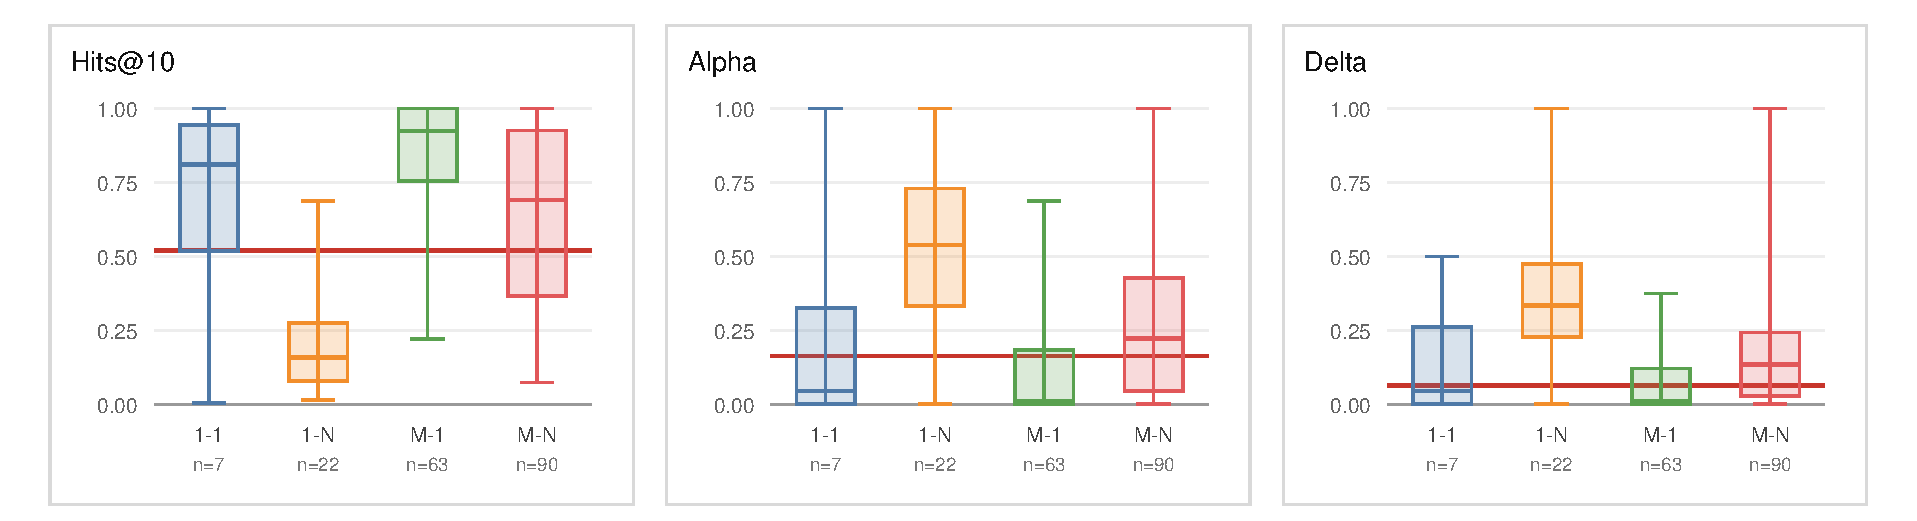
\includegraphics[width=0.86\textwidth]{figures/chap5/mapping-type/rotate-tail.pdf}
    \caption{RotatE mapping-type results for tail prediction. The red line
    marks the mean over all retained relations.}
    \label{fig:mapping-rotate-tail}
\end{figure}

The RotatE tail-prediction results are shown in
Figure~\ref{fig:mapping-rotate-tail}, which presents the clearest contrast
among the four mapping types.
The \(1\)-\(N\) group has the lowest Hits@10 and the highest
\(\alpha\) and \(\delta\). Its tail predictions are therefore less accurate and
show more hit-or-miss disagreement across the repeated RotatE runs. The
\(M\)-\(1\) group is at the other end of the comparison: it has the highest
Hits@10 and the lowest \(\alpha\) and \(\delta\). Taken together, these results
suggest that predictive multiplicity varies across mapping types in RotatE tail
prediction.

\begin{figure}[!t]
    \centering
    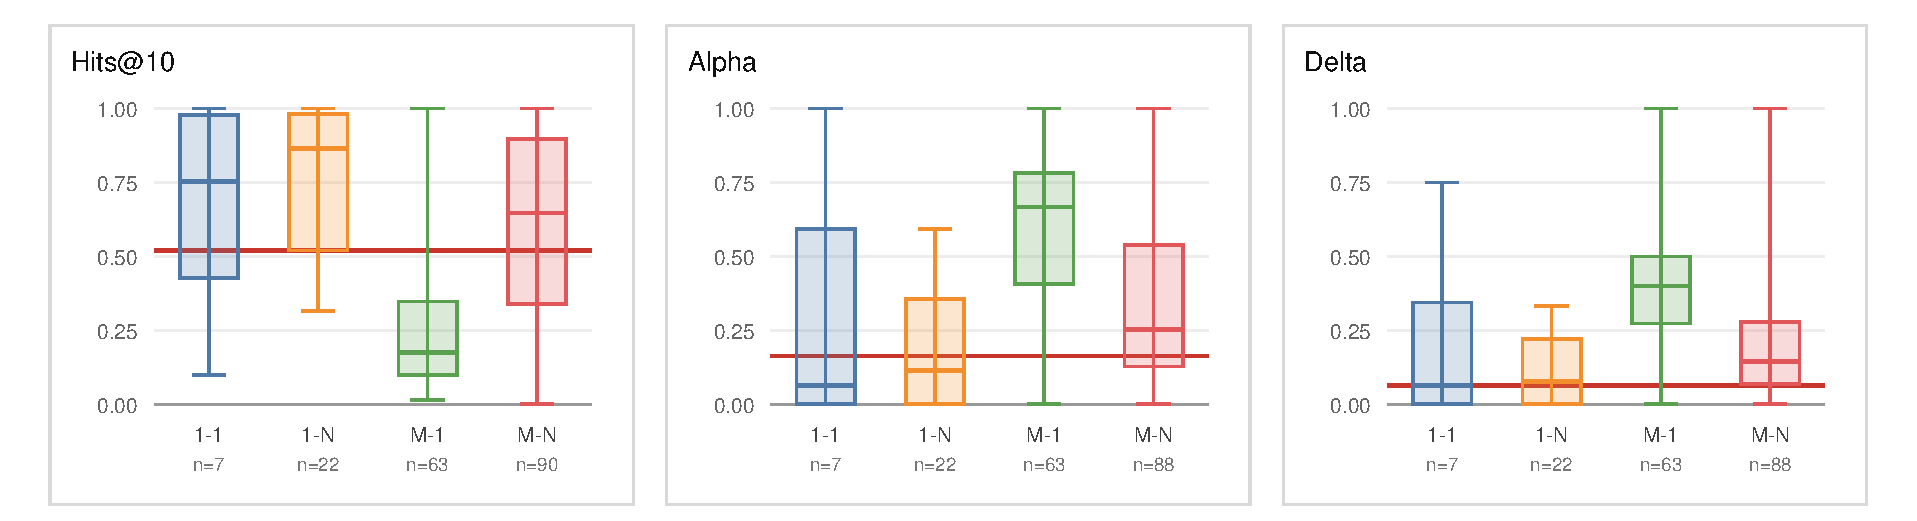
\includegraphics[width=0.86\textwidth]{figures/chap5/mapping-type/rotate-head.pdf}
    \caption{RotatE mapping-type results for head prediction. The red line
    marks the mean over all retained relations.}
    \label{fig:mapping-rotate-head}
\end{figure}

Figure~\ref{fig:mapping-rotate-head} shows a different pattern for head
prediction. The \(M\)-\(1\) group now has the lowest Hits@10 and the highest
\(\alpha\) and \(\delta\), while the \(1\)-\(N\) group has the highest Hits@10
and the lowest multiplicity measures. The relation group with lower accuracy
and higher multiplicity therefore changes when the prediction side changes.

\subsubsection{TransE Results}

The same side-aware comparison is also applied to TransE. The purpose of this
comparison is to check whether the directional pattern observed for RotatE also
appears under a different KGE model family.

\begin{figure}[!t]
    \centering
    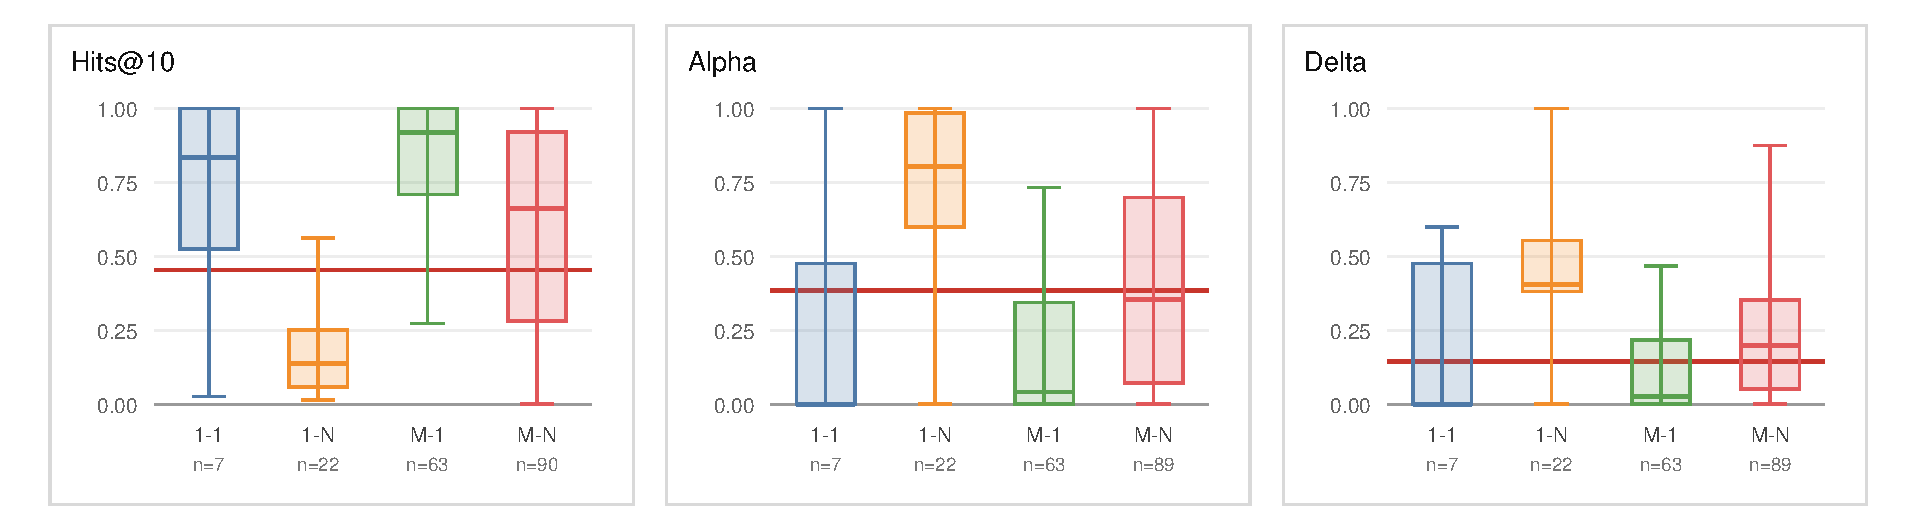
\includegraphics[width=0.86\textwidth]{figures/chap5/mapping-type/transe-tail.pdf}
    \caption{TransE mapping-type results for tail prediction. The red line
    marks the mean over all retained relations.}
    \label{fig:mapping-transe-tail}
\end{figure}

Although TransE is a different model family, its tail-prediction result shows
the same contrast between \(1\)-\(N\) and \(M\)-\(1\). In
Figure~\ref{fig:mapping-transe-tail}, the \(1\)-\(N\) group again has the
lowest Hits@10 and the highest \(\alpha\) and \(\delta\), whereas the
\(M\)-\(1\) group has the highest Hits@10 and the lowest multiplicity measures.
The lower accuracy and higher instability of the \(1\)-\(N\) tail side are
therefore observed in both models.

\begin{figure}[!t]
    \centering
    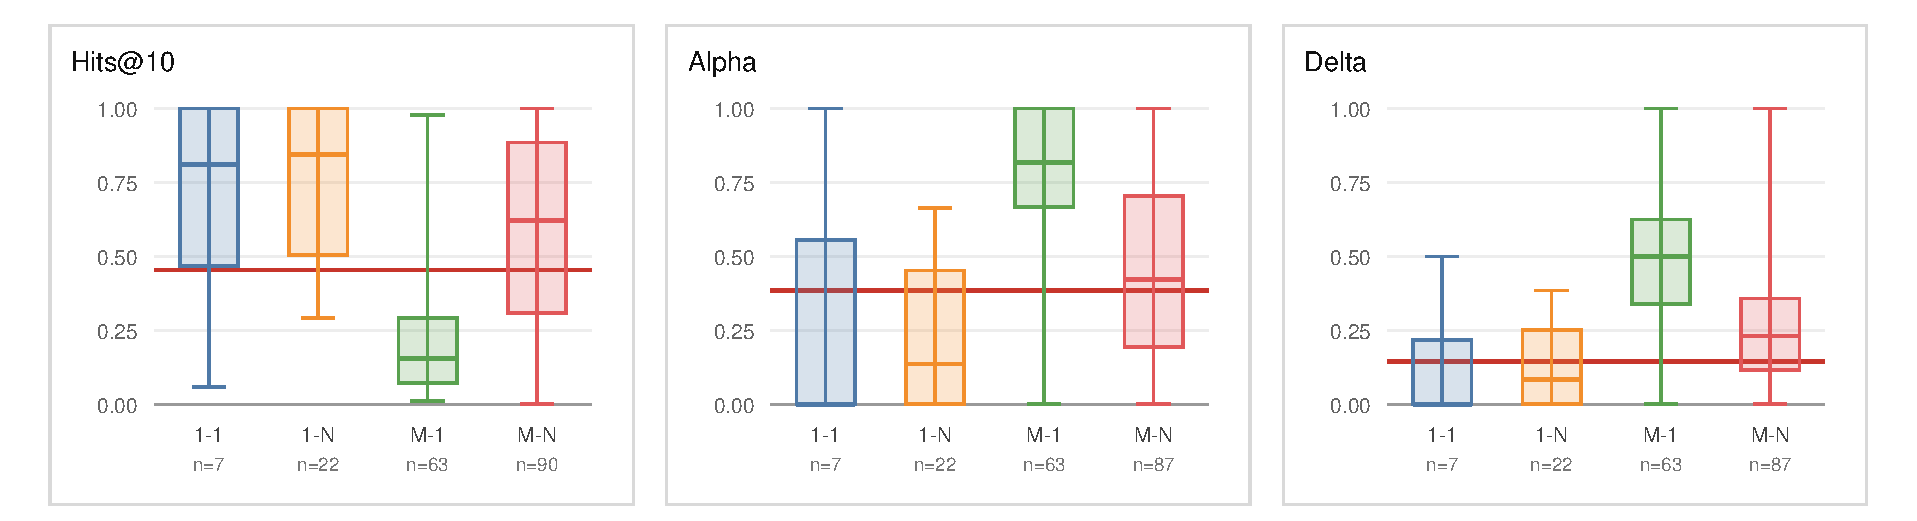
\includegraphics[width=0.86\textwidth]{figures/chap5/mapping-type/transe-head.pdf}
    \caption{TransE mapping-type results for head prediction. The red line
    marks the mean over all retained relations.}
    \label{fig:mapping-transe-head}
\end{figure}

Figure~\ref{fig:mapping-transe-head} completes the same reversal for head
prediction. The \(M\)-\(1\) group has the lowest Hits@10 and the highest
\(\alpha\) and \(\delta\). Compared with this group, the \(1\)-\(N\) group has
much higher Hits@10 and lower multiplicity measures. This agrees with the
RotatE head-prediction result.

A possible explanation is the set of constraints created by the training
triples. For a \(1\)-\(N\) relation, one fixed \((h,r)\) pair is connected to
several tail entities. Different training runs can represent or rank these
targets differently while retaining similar overall performance. This may lead
to higher \(\alpha\) and \(\delta\).

For an \(M\)-\(1\) relation, the constraints on tail prediction have a
different form. Triples such as \((h_1,r,t)\), \((h_2,r,t)\), and
\((h_3,r,t)\) provide several training constraints involving the same tail
entity, but each constraint belongs to a different tail query. The many-valued
structure is therefore on the head side rather than on the predicted tail side.
The same reasoning applies in reverse to head prediction, where a fixed
\((r,t)\) pair in an \(M\)-\(1\) relation is connected to multiple possible
head entities.

Under filtered evaluation, other known true answers are removed before the
candidate ranking is evaluated. The observed difference is therefore not
simply caused by known answers competing directly in the candidate list. The
four figures suggest that the constraints learned from the many side of
a relation leave more room for repeated runs to produce different ranking
decisions. This interpretation is consistent with the observed results, but
the current experiment does not test this training mechanism separately.

Overall, RotatE and TransE show the same side-dependent pattern on FB15k-237.
For \(1\)-\(N\) and \(M\)-\(1\) relations, predicting the side classified as
many is associated with lower accuracy and higher predictive multiplicity than
predicting the opposite side. This result suggests that the relation between
mapping type and predictive multiplicity depends on which side is predicted.

Tables~\ref{tab:mapping-type-tail-summary}
and~\ref{tab:mapping-type-head-summary} report the corresponding grouped means
for tail and head prediction.

\begin{table}[!t]
    \centering
    \caption{Relation-level means for tail prediction under
    \(\texttt{test\_support}\geq 10\).}
    \label{tab:mapping-type-tail-summary}
    \small
    \begin{tabular}{llrrr}
        \toprule
        Model & Mapping type & Hits@10 & \(\alpha\) & \(\delta\) \\
        \midrule
        RotatE & \(1\)-\(1\) & 0.6771 & 0.2422 & 0.1529 \\
        RotatE & \(1\)-\(N\) & 0.2104 & 0.5234 & 0.3659 \\
        RotatE & \(M\)-\(1\) & 0.8251 & 0.1076 & 0.0731 \\
        RotatE & \(M\)-\(N\) & 0.6313 & 0.2646 & 0.1591 \\
        TransE & \(1\)-\(1\) & 0.7016 & 0.2790 & 0.2218 \\
        TransE & \(1\)-\(N\) & 0.1741 & 0.7147 & 0.4596 \\
        TransE & \(M\)-\(1\) & 0.8180 & 0.1809 & 0.1117 \\
        TransE & \(M\)-\(N\) & 0.6065 & 0.3877 & 0.2200 \\
        \bottomrule
    \end{tabular}
\end{table}

\begin{table}[!t]
    \centering
    \caption{Relation-level means for head prediction under
    \(\texttt{test\_support}\geq 10\).}
    \label{tab:mapping-type-head-summary}
    \small
    \begin{tabular}{llrrr}
        \toprule
        Model & Mapping type & Hits@10 & \(\alpha\) & \(\delta\) \\
        \midrule
        RotatE & \(1\)-\(1\) & 0.6664 & 0.3216 & 0.2145 \\
        RotatE & \(1\)-\(N\) & 0.7527 & 0.1939 & 0.1168 \\
        RotatE & \(M\)-\(1\) & 0.2836 & 0.5855 & 0.3835 \\
        RotatE & \(M\)-\(N\) & 0.5971 & 0.3366 & 0.1994 \\
        TransE & \(1\)-\(1\) & 0.6861 & 0.3015 & 0.1332 \\
        TransE & \(1\)-\(N\) & 0.7455 & 0.2261 & 0.1339 \\
        TransE & \(M\)-\(1\) & 0.2439 & 0.7523 & 0.4893 \\
        TransE & \(M\)-\(N\) & 0.5764 & 0.4355 & 0.2474 \\
        \bottomrule
    \end{tabular}
\end{table}

\subsection{Inverse Relation Analysis}
\label{sec:inverse_analysis}

\subsubsection{Motivation}

When two relations form an inverse pair, they describe the connection between
the same entities in opposite directions. Training edges under the two
relations can therefore provide paired structural evidence: one relation
supports the connection from the head to the tail, while its inverse partner
supports the reversed connection. Such evidence may constrain the relation
representations learned under different random seeds and make their ranking
decisions more stable.

The analysis uses the inverse clarity defined in
Chapter~\ref{chap:framework}. This score measures whether the strongest mutual
inverse partner of a relation is clearly separated from its second-best
partner. A high value therefore indicates both substantial reverse support and
a clearly identified inverse partner. For readability, the tables in this
section use \emph{score} as a shorter name for inverse clarity.

\subsubsection{Results}

Table~\ref{tab:inverse-spearman} reports the global Spearman correlations
between the inverse score and the three relation-level evaluation metrics.
Across all relations, the inverse score does not show a monotonic association
with improved accuracy or stability. For RotatE and TransE, the Spearman
correlations with Hits@10 are \(-0.2796\) and \(-0.2819\), respectively. The
corresponding correlations with \(\alpha\) and \(\delta\) are positive and
range from \(0.2263\) to \(0.2427\). These global correlations therefore do
not indicate a general accuracy or stability benefit as the inverse score
increases.

\begin{table}[!t]
    \centering
    \caption{Spearman correlations between inverse clarity and relation-level
    Hits@10, \(\alpha\), and \(\delta\).}
    \label{tab:inverse-spearman}
    \small
    \begin{tabular}{lrrr}
        \toprule
        Model & Spearman (Hits@10) & Spearman (\(\alpha\)) &
        Spearman (\(\delta\)) \\
        \midrule
        RotatE & -0.2796 & 0.2398 & 0.2263 \\
        TransE & -0.2819 & 0.2371 & 0.2427 \\
        \bottomrule
    \end{tabular}
\end{table}

The global correlations do not show a monotonic benefit across all relations.
However, the score-group comparison in
Table~\ref{tab:inverse-score-groups} reveals a distinct pattern at the upper
end of the inverse-score distribution. The five relations with scores above
\(0.5\) show the clearest positive result. For RotatE, mean Hits@10 reaches
\(0.8000\), compared with \(0.5797\) across all retained relations, while both
\(\alpha\) and \(\delta\) fall to \(0\). For TransE, mean Hits@10 reaches
\(0.6866\), compared with the overall mean of \(0.5585\), while \(\alpha\) and
\(\delta\) decrease from the overall means of \(0.3357\) and \(0.1885\) to
\(0.1361\) and \(0.0813\), respectively. In the current experiment, relations
with a strong and clearly identified inverse partner are therefore associated
with higher accuracy and substantially lower predictive multiplicity in both
models. The lower score ranges do not show a gradual improvement: relations in
\((0,0.5]\) have lower Hits@10 and higher multiplicity than those with a score
of zero.

\begin{table}[!t]
    \centering
    \caption{Relation-level results grouped by inverse clarity. The label
    \emph{Score} in the table refers to the inverse clarity defined in
    Chapter~\ref{chap:framework}.}
    \label{tab:inverse-score-groups}
    \small
    \begin{tabular}{llrrrr}
        \toprule
        Model & Score range & Relations & Hits@10 & \(\alpha\) & \(\delta\) \\
        \midrule
        RotatE & All relations & 182 & 0.5797 & 0.2433 & 0.1427 \\
        \cmidrule(lr){1-6}
        RotatE & Score \(=0\) & 78 & 0.6700 & 0.1721 & 0.1031 \\
        RotatE & \(0<\text{Score}\leq 0.5\) & 99 & 0.4974 & 0.3116 & 0.1812 \\
        RotatE & Score \(>0.5\) & 5 & 0.8000 & 0.0000 & 0.0000 \\
        \midrule
        TransE & All relations & 182 & 0.5585 & 0.3357 & 0.1885 \\
        \cmidrule(lr){1-6}
        TransE & Score \(=0\) & 78 & 0.6480 & 0.2565 & 0.1452 \\
        TransE & \(0<\text{Score}\leq 0.5\) & 99 & 0.4816 & 0.4082 & 0.2281 \\
        TransE & Score \(>0.5\) & 5 & 0.6866 & 0.1361 & 0.0813 \\
        \bottomrule
    \end{tabular}
\end{table}

One possible interpretation is that partial or ambiguous reverse support is
not sufficient to provide a consistent paired constraint. When the inverse
score is high, the reverse evidence is concentrated on a strong and clearly
separated partner, which may reduce variation across repeated runs. Although
the high-score range contains only five relations, the same pattern of higher
accuracy and lower predictive multiplicity appears in both RotatE and TransE.

\subsection{Symmetry Analysis}
\label{sec:symmetry_analysis}

\subsubsection{Motivation}

For a symmetric relation, an entity pair can be connected by the same relation
in both directions. The two endpoint entities can therefore occupy compatible
roles under that relation, and the training graph provides structural evidence
for both directional orderings. This may reduce the distinction between the
head and tail roles and make predictions less sensitive to differences between
repeated runs.

As discussed in Chapter~\ref{chap:framework}, the raw symmetry score can be
inflated by self-loop triples because a self-loop is identical to its reversed
edge. The following analysis therefore uses the symmetry score that excludes
self-loops, \(\operatorname{Sym}^{\neg\mathrm{loop}}(r)\). The shorter label
\emph{Score} in the tables refers to this excluding-self-loop score.

\subsubsection{Results}

The global correlations in Table~\ref{tab:symmetry-spearman} do not show a
clear monotonic association. For both models, the correlation between the
excluding-self-loop symmetry score and Hits@10 is close to zero. The
correlations with \(\alpha\) and \(\delta\) are also weak. Thus, the symmetry
score does not provide a global explanation of either predictive performance or
multiplicity.

\begin{table}[!t]
    \centering
    \caption{Spearman correlations between the excluding-self-loop symmetry
    score and relation-level Hits@10, \(\alpha\), and \(\delta\).}
    \label{tab:symmetry-spearman}
    \small
    \begin{tabular}{lrrr}
        \toprule
        Model & Spearman (Hits@10) & Spearman (\(\alpha\)) &
        Spearman (\(\delta\)) \\
        \midrule
        RotatE & 0.0122 & 0.1310 & 0.1292 \\
        TransE & 0.0117 & 0.0425 & 0.0520 \\
        \bottomrule
    \end{tabular}
\end{table}

In Table~\ref{tab:symmetry-score-groups}, Hits@10 falls in the middle score
range and returns to slightly above the zero-score level in the high-score
range for both models. The multiplicity results are less consistent. In the
high-score range, both \(\alpha\) and \(\delta\) remain higher than those of the
zero-score relations. From the middle to the high-score range, they increase
slightly for RotatE but decrease for TransE. Higher symmetry scores are
therefore not consistently associated with lower predictive multiplicity.

\begin{table}[!t]
    \centering
    \caption{Relation-level results grouped by the excluding-self-loop
    symmetry score.}
    \label{tab:symmetry-score-groups}
    \small
    \begin{tabular}{llrrrr}
        \toprule
        Model & Score range & Relations & Hits@10 & \(\alpha\) & \(\delta\) \\
        \midrule
        RotatE & All relations & 182 & 0.5797 & 0.2433 & 0.1427 \\
        \cmidrule(lr){1-6}
        RotatE & Score \(=0\) & 164 & 0.5815 & 0.2294 & 0.1331 \\
        RotatE & \(0<\text{Score}\leq 0.5\) & 6 & 0.5047 & 0.3610 & 0.2236 \\
        RotatE & Score \(>0.5\) & 12 & 0.5924 & 0.3735 & 0.2341 \\
        \midrule
        TransE & All relations & 182 & 0.5585 & 0.3357 & 0.1885 \\
        \cmidrule(lr){1-6}
        TransE & Score \(=0\) & 164 & 0.5605 & 0.3307 & 0.1838 \\
        TransE & \(0<\text{Score}\leq 0.5\) & 6 & 0.4725 & 0.4436 & 0.2736 \\
        TransE & Score \(>0.5\) & 12 & 0.5742 & 0.3512 & 0.2119 \\
        \bottomrule
    \end{tabular}
\end{table}

A possible explanation is that symmetry places only a broad constraint on the
answer space. If a relation often appears in both directions, the entities on
its two sides are likely to have similar semantic roles. This may help the
model rule out clearly unsuitable candidates and may explain the slightly
higher Hits@10 in the high-score range. Symmetry still does not distinguish
among candidates that fit the same broad constraint. Different runs may still
rank these candidates differently, which may explain why \(\alpha\) and
\(\delta\) in the high-score range remain above those of the zero-score
relations. However, this explanation does not account for the lower Hits@10 in
the six-relation middle range, which remains unclear.

\section{Conclusion}
\label{chap:conclusion}

This thesis examined predictive multiplicity in knowledge graph embedding
based link prediction from a relation-level perspective. Using FB15k-237 and
repeated runs of RotatE and TransE, we compared relation-level Hits@10,
ambiguity, and discrepancy across mapping type, inverse score, and symmetry.
The clearest result was the association between mapping type and predictive
multiplicity. Across both models, relations with a one-to-many mapping in
either direction were less accurate and showed higher predictive multiplicity
when the many side was predicted. The inverse score did not have a monotonic
relation with accuracy or multiplicity. Although the high-score group contained
only a small number of relations, it showed higher accuracy and substantially
lower predictive multiplicity in both models. Symmetry showed no clear
association with predictive multiplicity.

The current experiments considered FB15k-237 and two KGE model families.
Future work could expand the set of comparable models and test whether the
same relation-level differences appear in other model families and datasets.
This thesis focused on identifying where predictive multiplicity occurs across
relations rather than reducing it. A further step is to use these findings to
develop methods that reduce instability in the relations and prediction
directions where it is most pronounced.


\Appendix
\section{Appendix}
\label{chap:appendix}

\subsection{Mapping-Type Grouped Means}
\label{app:mapping-type-tables}

Tables~\ref{tab:mapping-type-tail-summary}
and~\ref{tab:mapping-type-head-summary} report the grouped means corresponding
to the side-aware mapping-type figures in
Section~\ref{sec:mapping_type_analysis}.

\begin{table}[H]
    \centering
    \caption{Relation-level means for tail prediction under
    \(\texttt{test\_support}\geq 10\).}
    \label{tab:mapping-type-tail-summary}
    \small
    \begin{tabular}{llrrr}
        \toprule
        Model & Mapping type & Hits@10 & \(\alpha\) & \(\delta\) \\
        \midrule
        RotatE & \(1\)-\(1\) & 0.6771 & 0.2422 & 0.1529 \\
        RotatE & \(1\)-\(N\) & 0.2104 & 0.5234 & 0.3659 \\
        RotatE & \(M\)-\(1\) & 0.8251 & 0.1076 & 0.0731 \\
        RotatE & \(M\)-\(N\) & 0.6313 & 0.2646 & 0.1591 \\
        TransE & \(1\)-\(1\) & 0.7016 & 0.2790 & 0.2218 \\
        TransE & \(1\)-\(N\) & 0.1741 & 0.7147 & 0.4596 \\
        TransE & \(M\)-\(1\) & 0.8180 & 0.1809 & 0.1117 \\
        TransE & \(M\)-\(N\) & 0.6065 & 0.3877 & 0.2200 \\
        \bottomrule
    \end{tabular}
\end{table}

\begin{table}[H]
    \centering
    \caption{Relation-level means for head prediction under
    \(\texttt{test\_support}\geq 10\).}
    \label{tab:mapping-type-head-summary}
    \small
    \begin{tabular}{llrrr}
        \toprule
        Model & Mapping type & Hits@10 & \(\alpha\) & \(\delta\) \\
        \midrule
        RotatE & \(1\)-\(1\) & 0.6664 & 0.3216 & 0.2145 \\
        RotatE & \(1\)-\(N\) & 0.7527 & 0.1939 & 0.1168 \\
        RotatE & \(M\)-\(1\) & 0.2836 & 0.5855 & 0.3835 \\
        RotatE & \(M\)-\(N\) & 0.5971 & 0.3366 & 0.1994 \\
        TransE & \(1\)-\(1\) & 0.6861 & 0.3015 & 0.1332 \\
        TransE & \(1\)-\(N\) & 0.7455 & 0.2261 & 0.1339 \\
        TransE & \(M\)-\(1\) & 0.2439 & 0.7523 & 0.4893 \\
        TransE & \(M\)-\(N\) & 0.5764 & 0.4355 & 0.2474 \\
        \bottomrule
    \end{tabular}
\end{table}


\bibliographystyle{icml2025}   % 文献スタイルの指定
% \bibliographystyle{unsrt}
\bibliography{reference.bib}
%\bibliography{reference}        % 参考文献の出力

\end{document}
